\documentclass{beamer}
\usepackage[slovene]{babel}
\usepackage[utf8]{inputenc}
\usepackage[T1]{fontenc}
\usepackage{array}              %brez tega paketa ne bo delala točka: odkrivanje po stolpcih
\usepackage{palatino}
\usepackage{graphicx}
\usepackage{amsmath}
\usepackage{amsthm}
\usepackage{tikz}

\usepackage{relsize}

\beamertemplatenavigationsymbolsempty     %s tem ukazom skriješ gumbe za navigacijo


\usetheme{Berlin}
\usefonttheme{serif}
\usecolortheme{default}
\useinnertheme[shadows]{rounded}
\useoutertheme{infolines}

\newtheorem{definicija}{Definicija}
\newtheorem{izrek}{Izrek}
\newtheorem{trditev}[definicija]{Trditev}
\newtheorem{izrek_p_z}[izrek]{Izrek (Pearl in Paz)}
\newcommand{\cond}{\mathrel{\text{\scalebox{1.07}{$\perp\mkern-10mu\perp$}}}}



\title{Diplomski seminar}
   \subtitle{Modeliranje pogojne neodvisnosti s pomočjo grafov}
   \author{Jošt Gojkovič}
   \institute[FMF] {Fakulteta za matematiko in fiziko}
   \date{\today}                                               

\begin{document}




% ===================================================================
\begin{frame}
    \titlepage         %če tega ni, se un \title ne pokaže = naslovnica
  \end{frame}
  

% -------------------------------------------------------------------
\section{Motivacija}

\begin{frame}
    \frametitle{Grafično modeliranje}
    \begin{itemize}
        \item Grafični model ali verjetnostni grafični model je verjetnostni model, kjer z 
        grafi izrazimo pogojno odvisnost med slučajnimi spremenljivkami
        \item Povezave med vozlišči predstavljajo odvistnost
        \item Če je na primer povezava med vozliščem $A$ in $B$, to pomeni da je $A$ odvisen od $B$
        in $B$ od $A$. 
    \end{itemize}
   
\end{frame}

% -------------------------------------------------------------------
\section{Teorija Grafov}

\begin{frame}
    \frametitle{Notacija in terminologija}
    \begin{itemize}
        \item $G(V,E)$ enostaven graf, torej nima večkratnih povezav in zank. 
    \end{itemize}
    Večinoma bodo vozlišča označena, torej bodo razdeljena v 2 skupini.
    \begin{itemize}
        \item Množica vozlišč ima obliko 
        $$ V = \Delta \cup \Gamma \qquad \text{z} \qquad \Delta \cap  \Gamma = \emptyset  $$ 
        Pravimo, da so vozlišča v $\Delta$ diskretna, v $\Gamma$ pa zvezna.  
        \item Grafom z označenimi vozlišči pravimo označeni grafi 
    \end{itemize}
\end{frame}
% -------------------------------------------------------------------

\begin{frame}
    \frametitle{Notacija in terminologija}
    \begin{itemize}
        \item Poln graf je graf, v katerem vsaka povezava povezuje par njegovih točk,
        oziroma kjer so vse točke povezane vsaka z vsako.
        \item  Če je $A \subseteq V$, $A$ inducira podgraf $G_A = (A, E_A)$,
        kjer je $E_A = E \cap (A \times A)$ dobljena iz $G$ tako da ohranimo povezave z 
        začetnim in končnim vozliščem v $A$.
        \item Podmnožica je polna, če inducira poln podgraf
        \item Polni podmnožici, ki je maksimalna oziroma se je ne da povečat, pravimo klika
   
    \end{itemize}

\end{frame}
% -------------------------------------------------------------------
\begin{frame}
    \frametitle{Notacija in terminologija}
    \begin{itemize}
        \item Če imamo povezavo $ \alpha \longrightarrow \beta $, pravimo, da je $\alpha$ starš od $\beta$.
        Množica staršev vozlišča $\beta$ je označena s $pa(\beta)$.  
        \item Množico sosedov vozlišča $\alpha$ označimo z $ne(\alpha)$
        \item Oznaki $pa(A)$ in $ne(A)$ označujeta množico staršev in sosedov vozlišč v $A$,
        katera sama niso v $A$:
        \begin{align*}
              pa(A) = \cup_{\alpha \in A} pa(\alpha) \setminus A \\
              ne(A) = \cup_{\alpha \in A} pa(\alpha) \setminus A
        \end{align*}
        \item \emph{Meja} $bd(A)$ podmnožice vozlišč $A$ je množica vozlišč v $ V \setminus A $,
        ki so starši ali sosedi vozliščem v $A$. Torej $ bd(A) = pa(A) \cup ne(A)$. 
        \item \emph{Zaprtje} množice $A$ je $cl(A) = A \cup bd(A) $
    \end{itemize}

\end{frame}
% -------------------------------------------------------------------
\begin{frame}
    \frametitle{Notacija in terminologija}
    \begin{itemize}
        \item Množica $C \subseteq V $ je $ (\alpha, \beta)$-seperator, če vse poti od $\alpha$ do $\beta$ sekajo 
        množico $C$.
        \item $C \subseteq V $ separira $A$ od $B$, če je $ (\alpha, \beta)$-seperator za vse $\alpha \in A$
        in $\beta \in B$
    \end{itemize}
    \begin{definicija}
        Trojica $(A, B, C)$ disjunktnih podmnožic vozlišč neusmerjenega označenega garfa $G$ tvori
        močno dekompozicijo grafa $G$, če je $V = A \cup B \cup C$ in velja naslednje:
        \begin{enumerate}[(i)]
            \item $C$ separira $A$ od $B$
            \item $C$ je polna podmnožica množice $V$
            \item $C \subseteq \Delta \lor B \subseteq \Gamma$
        \end{enumerate}
    \end{definicija}
    \begin{itemize}
        \item Če pri enakih predpostavkah veljata samo 1. in 2. pogoj, potem trojica  $(A, B, C)$
        tvori šibko dekompozicijo.
        \item Pravimo, da $(A, B, C)$ dekompozira $G$ v komponenti $G_{A \cup C}$ 
        in $G_{B \cup C} $
    \end{itemize}

\end{frame}
% -------------------------------------------------------------------
\begin{frame}
    \frametitle{Pogojna neodvisnost}
    \begin{definicija}
        Slučajni spremenljivki $X$ in $Y$ sta pogojno neodvisni pri dani spremenljivki
        $Z$  če in samo če je pri dani vrednosti $Z$ verjetnostna porazdelitev $X$ enaka
        za vse vrednosti $Y$ in verjetnostna porazdelitev $Y$ je enaka za vse vrednosti
        $X$. Pišemo $ X \cond Y ~|~ Z $. 
    \end{definicija}
    Za drisketne slučajne spremenljivke se ta pogoj prevede na: 
    \begin{align*}
         P(X=x, Y=y ~|~ Z=z) = P(X=x~|~Z=z) \cdot P(Y=y~|~Z=z) 
    \end{align*} 
    V primeru zveznih slučajnih spremenljivk:
    \begin{align*}
        X \cond Y ~|~ Z \Longleftrightarrow  f_{XY|Z} (x,y|z) = f_{X|Z} (x|z) \cdot f_{Y|Z} (y|z)\\
    \end{align*}
\end{frame}
% -------------------------------------------------------------------
\begin{frame}
    \frametitle{Pogojna neodvisnost}
        Relacija $ X \cond Y ~|~ Z$ ima naslednje lastnosti: \newline \newline
        (C1) $\text{če} ~X \cond Y ~|~ Z~ \text{potem}~ Y \cond X ~|~ Z;$\newline \newline
        (C2) $\text{če} ~X \cond Y ~|~ Z~ \text{in} ~U = h(X) ~\text{potem}~ U \cond Y ~|~ Z;$\newline \newline
        (C3) $\text{če} ~X \cond Y ~|~ Z~ \text{in} ~U = h(X) ~\text{potem}~ X \cond Y ~|~ (Z,U);$\newline \newline
        (C4) $\text{če} ~X \cond Y ~|~ Z~ \text{in} ~X \cond W ~|~ (Y,Z) ~\text{potem}~ X \cond (W,Y) ~|~ Z.$\newline \newline
        V (C2) in (C3) je $h$ neka merljiva funkcija na vzorčnem prostoru od $X$.
        Ob dodatnih predpostavkah velja še (treba vprašat) \newline \newline
        (C5) če $ X \cond Y ~|~ Z$ in $ X \cond Z ~|~ Y$ potem $ X \cond (Y,Z)$ 
\end{frame}
% -------------------------------------------------------------------
\begin{frame}
    \begin{itemize}
        \item Zanimivo je, če si predstavljamo relacije $(C1)-(C5)$ kot izraze,
        ki niso nujno povezani z verjetnostjo, ampak z irelevanco oziroma nepomembnostjo.
        \item Pomebmen primer modela irelevance je seperacija grafov:
    \end{itemize}
    Označimo $A \perp B ~|~ C ~ \Longleftrightarrow ~ C ~\text{separira}~ A~ \text{od} ~B~ \text{v}~ G$ \\
    Potem ima seperacija grafov naslednje lastnosti:\newline \newline
    (C1) $\text{če} ~A \perp B ~|~ C~ \text{potem}~ B \perp A ~|~ C;$\newline \newline
    (C2) $\text{če} ~A \perp B ~|~ C~ \text{in} ~U \subseteq A ~\text{potem}~ U \perp B ~|~ C;$\newline \newline
    (C3) $\text{če} ~A \perp B ~|~ C~ \text{in} ~U \subseteq B ~\text{potem}~ A \perp B ~|~ (C \cup U);$\newline \newline
    (C4) $\text{če} ~A \perp B ~|~ C~ \text{in} ~A \perp D ~|~ (B \cup C) ~\text{potem}~ A \perp (B \cup D) ~|~ C.$\newline \newline
    Če so še vse množice disjunktne, velja še analogno od $C(5)$ 
\end{frame}
% -------------------------------------------------------------------
\begin{frame}
    \frametitle{Markove lastnosti na neusmerjenih grafih}
    \begin{itemize}
        \item Naj bo $V$ množica vozlišč grafa $G=(V,E)$
        \item Naj bodo $(X_\alpha)_{\alpha \in V}$ slučajne spremenljivke, ki zavzemajo vrednosti
        v verjetnostnih prostorih $(\mathcal{X}_\alpha)_{\alpha \in V}$. 
        \item Za $A \subseteq V$ naj bo $(\mathcal{X}_A) = \times_{\alpha \in A} ~ \mathcal{X}_\alpha$ in $\mathcal{X} = \mathcal{X}_V$
        \item označimo $X_A = (X_\alpha)_{\alpha \in A}$ 
        \item Uporabimo kratko notacijo $A \cond B ~|~ C$ za $X_A \cond X_B ~|~ X_C$
    \end{itemize}
\end{frame}
% -------------------------------------------------------------------

\begin{frame}
    \frametitle{Markove lastnosti na neusmerjenih grafih}
    Naj bo $G = (V,E)$ neusmerjen graf in naj bodo $ (X_\alpha)_{\alpha \in V} $
    slučajne spremenljive. Pravimo, da verjetnostna mera $P$ na $\mathcal{X}$ zadošča: 
    \newline \newline
    $(P) \quad $\emph{Pairwise Markovi lastnosti} glede na $G$ če je za 
    vsak par nesosednjih vozlišč $(\alpha, \beta)$: 
    $$ \alpha \cond \beta ~|~ V \setminus \{\alpha, \beta\}   $$

    $(L) \quad $ \emph{Lokalni Markovi lastnosti} glede na $G$, če je za 
    vsako vozlišče $\alpha \in V$:
    $$ \alpha \cond V \setminus cl(\alpha) ~|~ bd(\alpha) $$ 

    $(G) \quad $ \emph{Globalni Markovi lastnosti} glede na $G$, če je za 
    vsako trojico $(A, B, S)$ disjunktnih podmnožic $V$, tako da $S$ 
    separira $A$ od $B$ v $G$:
    \[ A \cond B ~|~ S \] 

\end{frame}
% -------------------------------------------------------------------
\begin{frame}
    \begin{trditev}
        Za vsak neusmerjen graf $G$ in vsako verjetnostno porazdelitev na $\mathcal{X}$ velja:
        $$ (G) \Longrightarrow (L) \Longrightarrow (P) $$
    \end{trditev}
    Ob predpostavki, da za disjunktne podmnožice $A$, $B$, $C$ in $D$ velja
    $$(1) \quad \text{če} ~A \cond B ~|~ (C \cup D) ~\text{in}~ A \cond C ~|~ (B \cup D) ~ \text{potem} ~ A \cond (B \cup C) ~|~ D $$
    imamo naslednji izrek:
    \begin{izrek_p_z}
        Če je verjetnostna porazdelitev na $\mathcal{X} $ taka, da velja $(1)$ za disjunktne
        podmnožice $A$, $B$, $C$, $D$, potem 
        $$ (G) \Longleftrightarrow (L) \Longleftrightarrow (P)$$
    \end{izrek_p_z}
\end{frame}

% -------------------------------------------------------------------
\begin{frame}
    \frametitle{Zgled (disketna porazdelitev)}
    Naj bodo $(X,Y,Z)$ porazdeljene enako $X=Y=Z$ s $P\{X=0\} = P\{X=1\} = \frac{1}{2}. $
    Ta porazdelitev potem ustreza parni Markovi lastnosti $(P)$.\\
    \begin{align*}
        
    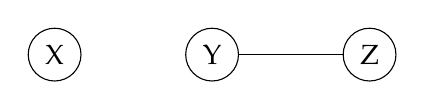
\begin{tikzpicture}
        \node[shape=circle,draw=black] (X) at (3,0) {X};
        \node[shape=circle,draw=black] (Y) at (5,0) {Y};
        \node[shape=circle,draw=black] (Z) at (7,0) {Z};
        \path [-] (Y) edge node[left] {} (Z);
    \end{tikzpicture}
    \end{align*}
\end{frame}
% -------------------------------------------------------------------
\begin{frame}
    \frametitle{Zgled (normalna porazdelitev)}
    Naj bo $Y = (Y_1, Y_2, Y_3)^T$, $Y \sim \mathcal{N} (0,\Sigma)$ s kovariančna matriko
    \begin{equation*}
    \Sigma =
    \begin{pmatrix}
        1 & \frac{1}{\sqrt{n}} & \frac{1}{2}\\
        \frac{1}{\sqrt{n}} & \frac{2}{n} &\frac{1}{\sqrt{n}}\\
        \frac{1}{2} & \frac{1}{\sqrt{n}} & 1
    \end{pmatrix}	
\end{equation*}

Izkaže se, da je pogojna porazdelitev od $(Y_1, Y_3)^T$ pri danem $Y_2$ dvorazsežna normalna
s kovariančno matriko

\begin{equation*}
    \Sigma_{13|2} = 
    \begin{pmatrix}
        1 &  \frac{1}{2}\\
        \frac{1}{2} &  1
    \end{pmatrix}
    -
    \begin{pmatrix}
        \frac{1}{\sqrt{n}}\\
        \frac{1}{\sqrt{n}}
    \end{pmatrix}
    (\frac{n}{2}) \cdot (\frac{1}{\sqrt{n}}, \frac{1}{\sqrt{n}}) = 
    \begin{pmatrix}
        \frac{1}{2} &  0\\
        0 &  \frac{1}{2}
    \end{pmatrix}
\end{equation*}
in zato $Y_1 ~ \cond ~ Y_3 ~|~ Y_2$, kar pomeni, da $Y$ zadošča globalni Markovi lastnosti na grafu:
\begin{align*}
    
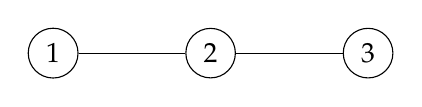
\begin{tikzpicture}
    \node[shape=circle,draw=black] (X) at (7,0) {1};
    \node[shape=circle,draw=black] (Y) at (9,0) {2};
    \node[shape=circle,draw=black] (Z) at (11,0) {3};
    \path [-] (Y) edge node[left] {} (Z);
    \path [-] (X) edge node[left] {} (Y);
\end{tikzpicture}
\end{align*}


\end{frame}

% -------------------------------------------------------------------

\end{document}